\begin{figure}
  \centering
  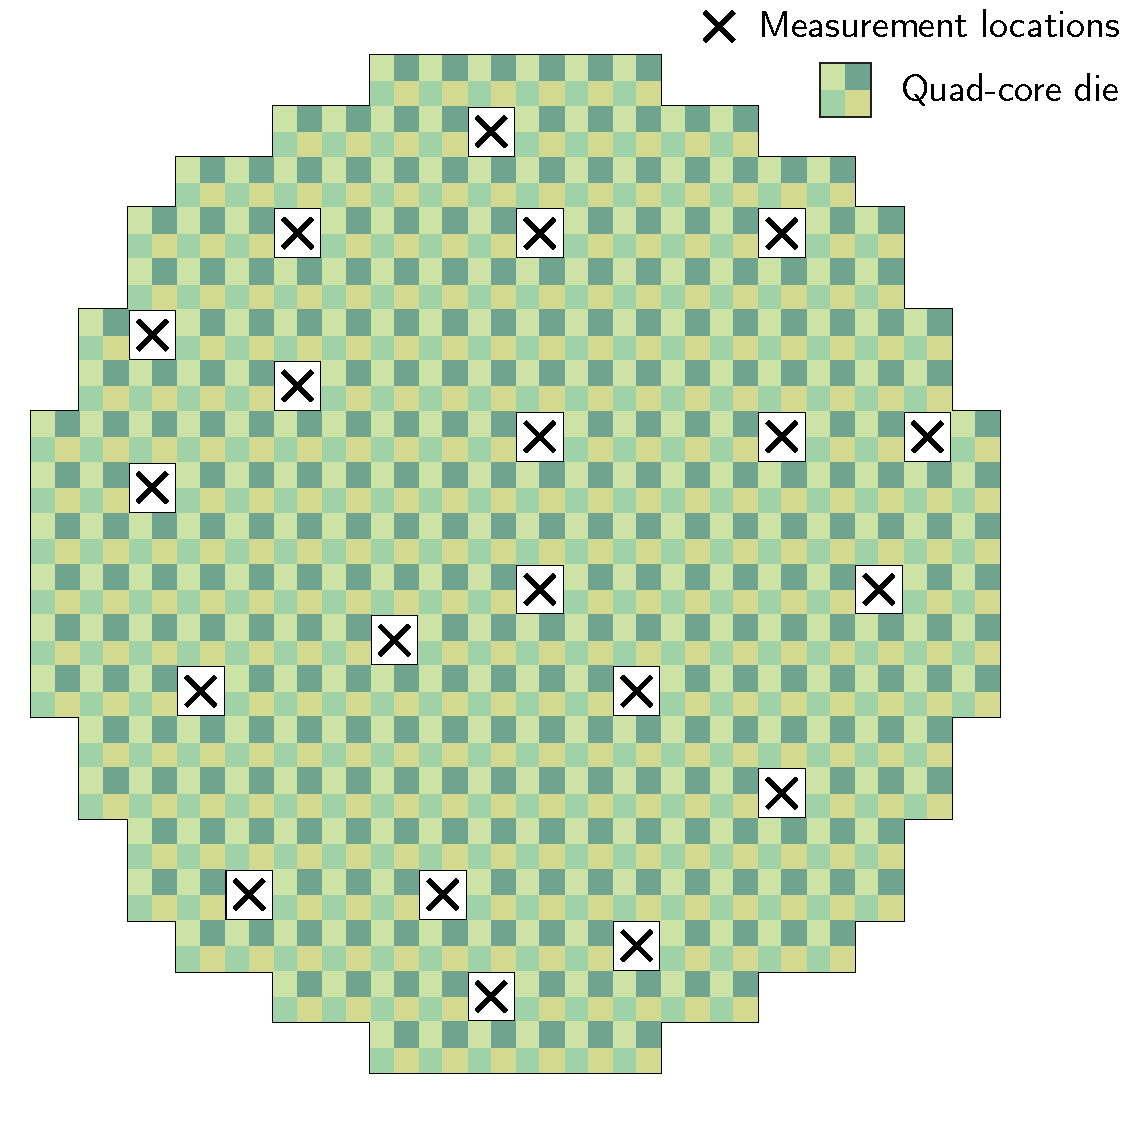
\includegraphics[width=0.7\linewidth]{include/assets/wafer-pick.pdf}
  \caption{A wafer with 316 quad-core dies.}
  \flabel{wafer-pick}
  \vspace{-1.5em}
\end{figure}

Consider a electric system that consists of $\nprocs$ power-dissipating components identified at the intended level of granularity (processors, ALUs, caches, registers, \etc); hereafter, these components are referred to as processing elements.
The system is being produced on a silicon wafer that hosts $\ndies$ dies (chips).
Let $\specification$ be the specification of the fabrication process that includes: (a) the layout of the wafer; (b) the floorplan of a single die of the wafer; (c) the thermal parameters of the materials that the system is made of.

A power profile $\profileP$ of a die is a tuple composed of a data matrix $\mP = (\vP_i) \in \real^{\nprocs \times \nsteps}$, $\vP_i \in \real^\nprocs$, that captures the power dissipation of all the $\nprocs$ processing elements at $\nsteps$ moments of time and a (column) vector $\partition{\mP} = (\t_i) \in \real^{\nsteps}$ with positive and strictly increasing components that specifies these moments of time.
The definition of a temperature profile $\profileT$ is the same as the one for power except that the data matrix $\mT = (\vT_i) \in \real^{\nprocs \times \nsteps}$, $\vT_i \in \real^\nprocs$, contains temperature.

The system is assumed to depend on a random element, denoted by $\u$, which manifests itself in deviations of the actual power dissipation from nominal values and, consequently, in deviations of temperature from the one corresponding to the nominal power consumption.
An important instantiation of such a random quantity is the effective channel length discussed earlier.
The goal of this work is to develop a framework for the characterization of the distribution of $\u$ across the wafer such that this framework possesses the following properties: (a) low deployment costs, (b) computational efficiency, (c) ability to operate on incomplete and noisy data, and (d) ability to accommodate the prior knowledge of the user.
To this end, we propose the use of indirect measurements. Specifically, we aim at measuring temperature, as described in \sref{motivation}, which we further analyze using the ideas originating from Bayesian inference.
The inputs to our framework are: (a) the specification of the fabrication process $\specification$, (b) a test workload given as a dynamic power profile $\profilePdyn$, and (c) a set of measured temperature profiles, corresponding to $\profilePdyn$, collected at several locations on the wafer. Denote by
\[
  \Data = \left\{ (\mT^{(i)}_\meas, \partition{\mT}), \r_i \right\}_{i = 1}^\nrdies
\]
such a data set composed of $\nrdies$ temperature profiles $(\mT^{(i)}_\meas, \partition{\mT})$ of $\nrdies$ out of $\ndies$ dies on the wafer and the corresponding spatial locations of these dies $\vr = (\r_i) \in \domain^\nrdies$ in the domain $\domain$ representing the surface of the wafer.
It is important to note that $\mT^{(i)}_\meas$ can potentially contain data only for a subset of the processing elements, say $\nrprocs \leq \nprocs$, and/or only for a subset of the time moments of the power partition $\partition{\mP}$, say $\nrsteps \leq \nsteps$; therefore, we let $\mT^{(i)}_\meas$ be in the space $\real^{\nrprocs \times \nrsteps}$.
For simplicity, the temperature profiles in $\Data$ are assumed to share the same subset of the measured processing elements and the same time partition.
The test power profile is assumed to be fine-grained whereas temperature profiles are presumably sparse, \ie, $\nrsteps \ll \nsteps$.
Since $\Data$ is assumed to be incomplete, the number of measured dies is typically much smaller than the total number of dies on the wafer, \ie, $\nrdies \ll \ndies$.
Finally, the output of the framework should be comprised of the probability distributions of $\u$ at an arbitrary set of spatial locations on the wafer chosen by the user.
